\section{Nicht Lineare Systeme}
\subsection{Basics}
\begin{itemize}
	\item Superpositionsprinzip gilt nicht
	\item Stabilität ist lokale Eigenschaft
	\item Finite Escape time (Wert in endlicher Zeit bei $\infty$)
	\item Viele Beharrungszustände
	\item Chaotische Systeme existieren
\end{itemize}
\subsection{Bestimmung der Stabilität}
\subsubsection{Layapunov 1. Methode}
\begin{itemize}
	\item System um Beharrungszustand linearisieren
	\begin{itemize}
		\item Stabilität im linearisierten System $\Rightarrow$ Stabilität um Beharrungszustand
	\end{itemize} 
	\item Sind die Realanteile der Eigenwerte  $< 0$ ist das System an dem Punkt stabil um den Beharrungszustand
	\item Sind die Realanteile der Eigenwerte  $> 0$ ist das System an dem Punkt instabil um den Beharrungszustand
	\item Siehe für Beispiel Gleichung \ref{eq:Layapunov1} (ist Aufgabe 1 aus \glqq Nicht lineare Systeme I\grqq)
	\item Linearisieren an einem Punkt, entspricht der Jacobi-Matrix mit den Werten dieses Punktes Eingesetzt $\rightarrow$ Matrix $A$
\end{itemize}
\begin{align}
	\label{eq:Layapunov1}
	\dot{\underline{x}} &= f(\underline{x})
	\begin{bmatrix}
		x_1\\
		x_2
	\end{bmatrix} = \begin{bmatrix}
		x_2\\
		-\frac{r}{m}x_2-\frac{g}{l}x\sin(x_1)
	\end{bmatrix}\\
	J &= \left.\begin{bmatrix}
		\frac{\partial f_1(x1,x2)}{\partial x1}	& \frac{\partial f_1(x1,x2)}{\partial x2}\\
		\frac{\partial f_2(x1,x2)}{\partial x1} &\frac{\partial f_2(x1,x2)}{\partial x2}
	\end{bmatrix}\right\lvert_{\begin{matrix}
		x_1\\x_2
	\end{matrix}}
\end{align}

\subsubsection{Layapunov 2. Methode}
\begin{itemize}
	\item Laypunov-Funktion $V(x)$, damit diese zulässig ist, müssen folgende Bedingungen erfüllt sein:
	\begin{itemize}
		\item []$V\left(\underline{0}\right) = 0$
		\item []$V\left(\underline{x}\right) > 0$
	\end{itemize}	
	\item Reminder: $\underline{x}$ sind Funktionen $\rightarrow$ Ableitung von $V(x)$ mit Kettenregel
	\begin{itemize}
		\item [z.B.] $V(\underline{x}) = x_1^2+x_2^2 \qquad\Rightarrow \dot{V}(x) = 2x_1\dot{x}_1 + 2x_2\dot{x}_2$
	\end{itemize}
	\item Ein System ist um einen Bereich (um $\underline{x}$)lokal stabil, wenn $\dot{V}\left(\underline{x}\right) < 0$ erfüllt ist 
\end{itemize}

\subsubsection{Layapunov in Linearen Systemen}
\begin{itemize}
	\item In Linearen System können folgende Abgewandelte Bedienungen angewendet werden, wenn folgendes erfüllt ist:
	\begin{itemize}
		\item $P>0 \rightarrow$ Positiv definite Matrix (alle Eigenwerte von $P>0$)
	\end{itemize}
	\item Gleichtung \ref{eq:Layapunov2} ist die Layapunov-Gleichung
\end{itemize}
\begin{align}
	V(x) &=x^TPx\\
	\dot{V}(x) &= x^TA^TPx+x^TPAx < 0\\
	\label{eq:Layapunov2}
	A^T+PA&=-Q\\
	Q&=B^TB	\qquad \text{Mass für Beobachtbarkeit}\\
	Q&=CC^T	\qquad	\text{Mass für Steuerbarkeit}
\end{align}

\subsection{Popov-Kreiskriterium}
\begin{itemize}
	\item Miteinkalkulieren einer Gewissen Nichtlinearität der Regelstrecke
	\begin{itemize}
		\item Begrenzt durch zwei Lineare Funktionen
	\end{itemize}
	\item Nichtlinearität darf keine Sprünge enthalten
	\item Nichtlinearität innerhalb eines Bereiches Eingrenzen
	\begin{itemize}
		\item Dieser Bereich wird mit zwei Steigungen beschrieben, $a$ und $b$
	\end{itemize}
	\item Das Popovkriterium ist eine Erweiterung des Nyquist-Kriterium
	\begin{itemize}
		\item In diesem Fall ist es ein Kreis, definiert durch die Steigungen der begrenzenden Funktionen
		\item Siehe für den Zusammenhang  Abbildung \ref{fig:Popov1} und \ref{fig:Popov3}
		\item Pro instabilem Pol muss die Frequenzlinie den Kreis einmal im Gegenuhrzeigersinn umkreisen, ohne die Fläche zu berühren.
	\end{itemize}
	\item Die Wichtigsten Sonderfälle sind in Abbildung \ref{fig:PopovSonderfaelle} gezeigt. 
\end{itemize}
\begin{figure}[!h]
	\footnotesize
	\begin{minipage}{0.25\linewidth}
		\footnotesize
		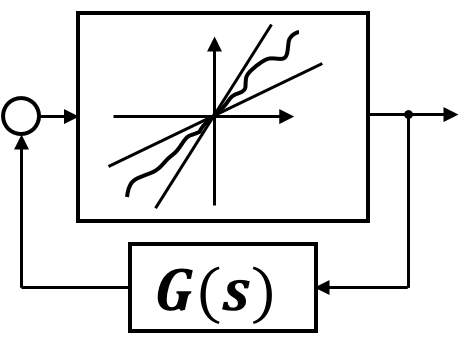
\includegraphics[width=1\linewidth]{./bilder/Popov2.png}
		\caption{Ersatzschaltbild von Popov}
	\end{minipage}\hspace{0.1\linewidth}
	\begin{minipage}{0.25\linewidth}
		\footnotesize
		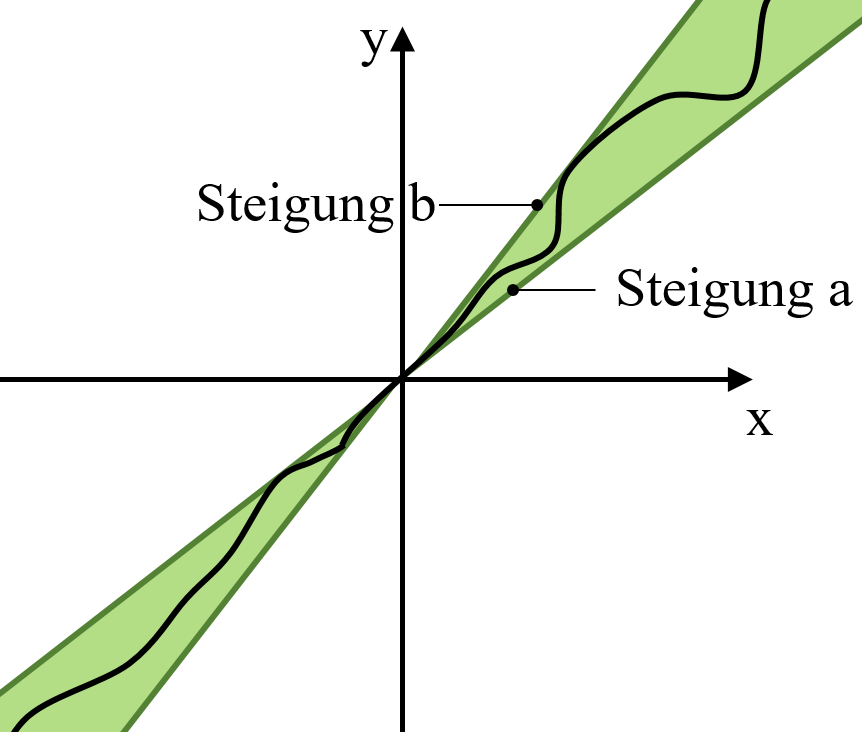
\includegraphics[width=1\linewidth]{./bilder/Popov1.png}
		\label{fig:Popov1}
		\caption{Begrenzende Funktionen umgeben die Nichtlinearität}
	\end{minipage}\hspace{0.1\linewidth}
	\begin{minipage}{0.25\linewidth}
		\footnotesize
		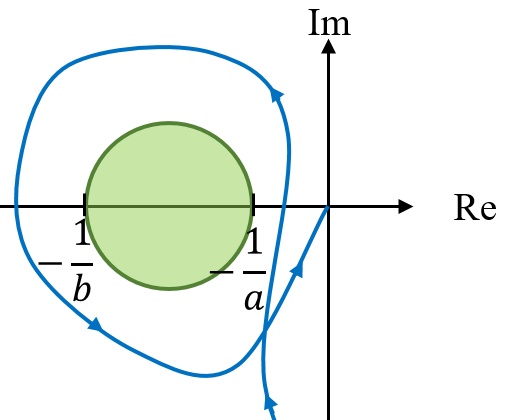
\includegraphics[width=1\linewidth]{./bilder/Popov3.png}
		\label{fig:Popov3}
		\caption{Zusammenhang zwischen begrenzenden Funktionen und Nyquist diagramm}
\end{minipage}
\end{figure}

\begin{figure}[!h]
	\centering
	\begin{minipage}{0.15\linewidth}
		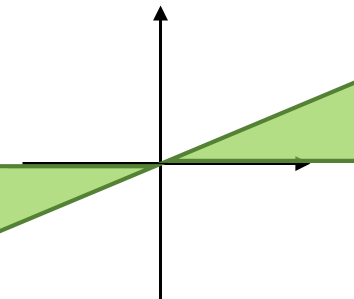
\includegraphics[width=1\linewidth]{./bilder/Popov4.png}.
	\end{minipage}\hspace{0.05\linewidth}$\Rightarrow$\hspace{0.05\linewidth}
	\begin{minipage}{0.15\linewidth}
		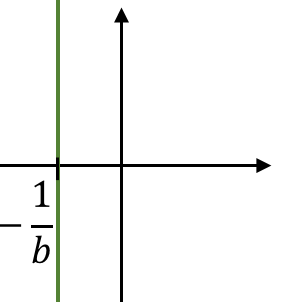
\includegraphics[width=1\linewidth]{./bilder/Popov5.png}.
	\end{minipage}\hspace{.1\linewidth}
	\begin{minipage}{0.15\linewidth}
		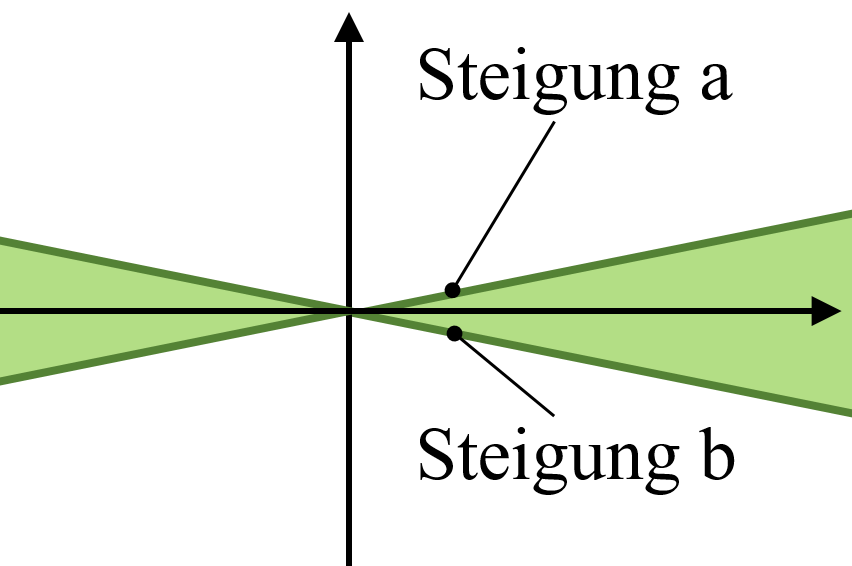
\includegraphics[width=1\linewidth]{./bilder/Popov6.png}.
	\end{minipage}\hspace{0.05\linewidth}$\Rightarrow$\hspace{0.05\linewidth}
	\begin{minipage}{0.15\linewidth}
		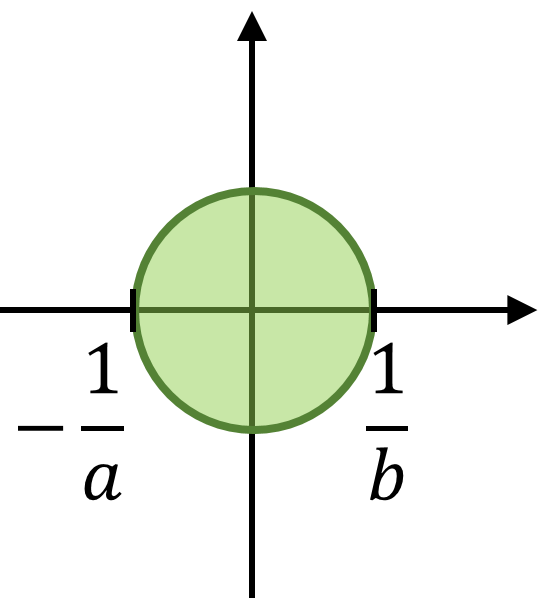
\includegraphics[width=1\linewidth]{./bilder/Popov7.png}.
	\end{minipage}	
	\label{fig:PopovSonderfaelle}
	\caption{Sonderfälle bei der Anwendung des Popov-Stabilitätskriterium}
\end{figure}

\subsection{Beschreibungsfunktionsmethode}
\begin{itemize}
	\item Beschreibungsfunktion wird mit $N(A)$ bezeichnet, siehe Anhang \ref{sec:AnhBeschreibungsf}
	\item Ziel: Die Beschreibungsfunktion beschreibt die Nichtlinearität des Systems
	\begin{itemize}
		\item Siehe Anhang für die wichtigsten Beschreibungsfunktionen
	\end{itemize}
	\item Totband:
	\begin{itemize}
		\item Erst wenn ein gewisser Fehler ($e$) Überschritten ist, passiert dieser das Totbandglied
		\item Der Ausgang nach dem Totband ist jeweils um 1/2 des Fehlers versetzt
		\item Gezeigt in Abbildung \ref{fig:totband}
	\end{itemize}
	\item Relais
	\begin{itemize}
		\item Schaltet jeweils bei 0-Durchgang des Eingangs
		\item Amplitude am Ausgang springt bei Nulldurchgang, auf die jeweilige Seite 
	\end{itemize}
\end{itemize}
\begin{figure}[!h]
	\centering
	\includegraphics[width=0.5\linewidth]{./bilder/totband.png}
	\label{fig:totband}
	\caption{Symbol des Totbandes und dessen Ein- und Ausgangssignal}
\end{figure}

\subsubsection{Grenzzyklus}
\begin{itemize}
	\item Regelkreis mit Maximaler Verstärkung 
	\item Phase ist \ang{-180}
	\item Der Grenzzyklus ist der Schnittpunkt gemäss Abbildung \ref{fig:Beschreibungsf}, gemäss Formel \ref{eq:Beschreibungsf1}
	\item Ein Grenzzyklus existiert, wenn
	\begin{itemize}
		\item die Linie der Beschreibungsfunktion im Nyquist-Diagramm schneidet die Frequenzlinie (des Open-Loops) von rechts nach links
		\item Dabei ist die Betrachtung aus sicht der zunehmenden Frequenz
		\item Siehe Beispiel in Abbildung \ref{fig:Beschreibungsf}
	\end{itemize}
	\item Es ist das $A$ gesucht, dies entspricht der Amplitude des Eingangssignal
	\begin{itemize}
		\item In diesem Fall $N(A)$ bestimmen mit Schnittpunkt und das $A$ ausrechnen
	\end{itemize}
	\item Oder die Grenzfrequenz ist gesucht
	\begin{itemize}
		\item Bestimmen durch Schnittpunkt gemäss Formel \ref{eq:Beschreibungsf1}
	\end{itemize}
	\item Oder die Zulässige Verstärkung des Regelkreises $\lvert G(j\omega)\rvert$ 
	\begin{itemize}
		\item Formel \ref{eq:Beschreibungsf1} auflösen nach $G(j\omega)$
	\end{itemize}
\end{itemize}

\begin{figure}[!h]
	\begin{minipage}{0.6\linewidth}
		\centering
		\includegraphics[width=.4\linewidth]{./bilder/Beschreibungsfunk1.png}
		\caption{Schnittpunkt ist bei der Grenzfrequenz, Beispiel für ein Relais}
		\label{fig:Beschreibungsf}
	\end{minipage}
	\begin{minipage}{0.3\linewidth}
		\begin{align}
		\label{eq:Beschreibungsf1}
		\frac{-1}{N(A)} = G_{Ol}(j\omega)
		\end{align}
	\end{minipage}
\end{figure}

\clearpage
\newpage